
\section{Seismicity of Northern Iran}
\label{sec:seismicity}

We are interested in applying the visibility graph method to analyze the seismicity of northern Iran. This region is part of the Iranian plateau, on the Himalayan-Alpine seismic belt. It is confined by the relative movements between the Arabian, Eurasian, eastern Asia-Minor, and Indian plates; and has a long history of large magnitude ($M>7$) earthquakes that are well documented dating back to the eight century \citep[e.g.,][]{Berberian_1981_Chap}. According to the tectonic settings and geologic provinces of the plateau, the seismic activity in Iran has been categorized into different seismic zones. These vary between four to nine major seismic zones, in the more traditional models \citep[e.g.,][]{Stocklin1968, Takin1972, Berberian1976}, and up to twenty to twenty-three seismotectonic provinces in the most elaborate ones \citep[e.g.,][]{Nowroozi1976, Tavakoli1999}. We adopt the model proposed by \citet{Mirzaei1998} with modifications introduced by \citet{Karimiparidari2013}. In it, Iran is divided into six seismic regions: Azerbaijan, Alborz, Kopeh Dagh, Zagros, Central-East Iran, and Makran. \myrevision{Each of these seismic regions, and in general, the whole Iranian plateau, have been the subject of various studies from different perspectives in the past \citep[e.g.,][]{Zafarani2017testing, Sedaghati2017partially, Golara2014, Nemati2015}. Here, our focus is on the northern part of the country,} for which we define a region of interest between longitudes 43.5\textdegree{}E and 61.5\textdegree{}E, and latitudes 34\textdegree{}N and 40\textdegree{}N, as shown in Fig.~\ref{fig:study_region}. Although this region encloses part of the Zagros and Central-East seismic zones, we limit our analysis to the seismicity of Azerbaijan, Alborz, and Kopeh Dagh.

\begin{figure*}[t]
	\centering
	\includegraphics[width=\textwidth]{figures/pdf/figure-02} 
	\caption{Region of interest, highlighting the seismic zones that are the focus of this study: Azerbaijan, Alborz, and Kopeh Dagh. The top-right location-map shows Iran and the selected area with respect to neighboring countries. The solid dark lines show the boundaries of the additional Zagros and Central-East seismic zones. This zonation follows the division proposed by \citet{Mirzaei1998} and later modified by \citet{Karimiparidari2013}. The background shows fault lines and the shaded relief.}
	\label{fig:study_region}
\end{figure*}

Northern Iran houses about 41 percent (32 million) of the total population of the country, and has suffered devastating earthquakes in the past \citep[e.g.,][]{Mehrain_1990_Tech, Chafory-Ashtiany_1999_DPM, Razzaghi_2012_Tech}. At the northwest, the seismic zone of Azerbaijan is strongly controlled by the North Tabriz Fault system in the vicinity of the city of Tabriz, shown in Fig.~\ref{fig:study_region}. Historical accounts document the occurrence of strong $M>6$ earthquakes in this region as far back as the ninth century \citep{Berberian1999}, and a few $M>7$ earthquakes in 1042, 1721, and 1780 \citep{Jones1834}. More recently, this region was struck by the $M_w$ 6.1 1997 Ardabil earthquake near the city of Ardabil, and the $M_w$ 6.4 2012 Tabriz earthquake northeast of the city of Tabriz. These earthquakes caused extensive damage and took the lives of more than 1,500 people. 

The seismicity in the north-central region of Alborz is dominated by multiple fault systems, including the Talesh, Rubdar, North Alborz, and North Tehran faults, which also have a history of producing strong ground shaking. According to \citet{Ambraseys_1982_Book}, Tehran was devastated by severe $M>7$ earthquakes in 743, 958, 1177, 1665, and 1830. This region has also seen some significant recent seismic activity \citep{Berberian1999}, including the $M_w$ 7.4 1990 Manjil-Rudbar earthquake, which caused numerous deaths and damage to the region in the south Caspian depression, south from the city of Rasht and northwest from Tehran. 

Last, there is the Kopeh Dagh seismic zone to the east and northeast. This region is dominated by the main Kopeh Dagh fault system, which exhibits active tectonic displacements along a distance of more than 500 km \citep{Trifonov1978}. This fault is responsible for the $M_w$ 7.3 1948 earthquake, which struck the capital city of Ashgabat in Turkmenistan and destroyed more than 30 villages in Iran. \myrevision{While no large magnitude events have been registered in recent years,} historically, the Kopeh Dagh seismic zone is responsible for the $M_s$ 7.1 earthquake in 10 A.D.~\citep{Berberian2001} near Ashgabat, and two significant earthquakes in 1209 and 1405 at the boundary between the Neyshabur and Binalud faults near the city of Mashhad \citep{Berberian1999}.

\begin{figure*}[t]
	\centering
	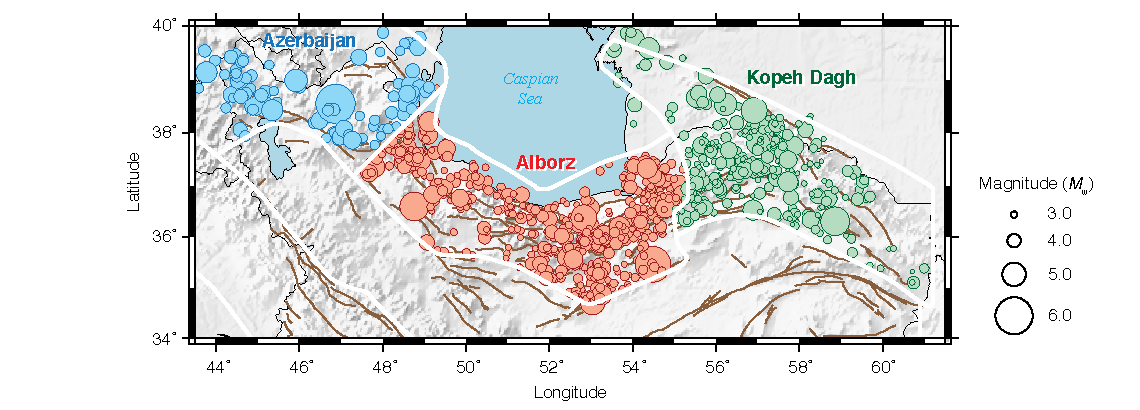
\includegraphics[width=\textwidth]{figures/pdf/figure-03} 
	\caption{\myrevision{Instrumental seismicity of northern Iran for the 2005--2016 period, considering only the events in the seismic zones of interest, namely Azerbaila, Alborz, and Kopeh Dagh, for the whole (a) and complete (b) catalogs.} The size of symbols are proportional to the magnitude of the events, as indicated by the artificial scale shown on the right. The background shows fault lines and the shaded relief.}
	\label{fig:seismicity}
\end{figure*}

It follows from this description that the region of interest is one of significant seismic activity, which goes back centuries. We are, however, interested in the most recent instrumental seismicity. In particular, we focus on events recorded in the last decade, between January 2005 and December \myrevision{2016}. We limit our analysis to this magnitude-time sequence period because in a previous study we observed that the latest decade of seismic records in northern Iran offered the most complete dataset of recorded events, especially for the case of small $M < 4$ earthquakes \citep{Khoshnevis2017}.

We compiled a catalog of all recorded earthquakes using data downloaded from the International Institute of Earthquake Engineering and Seismology, IIEES (\url{http://www.iiees.ac.ir/en/eqcatalog/}). \myrevision{In general, data collected from IIEES contains a mixture of earthquake magnitude scales, including: moment, $M_w$; local, $M_L$; body wave, $m_b$; surface wave, $M_s$; and duration $M_D$ magnitudes. However, for our time-period of interest (2005--2016), all the events had local magnitude ($M_L$) values, which we, in turn, and in order to maintain international consistency with other studies, converted to moment magnitude ($M_w$)} using the relationships defined in \citet{Zare2014}.

\myrevision{The whole dataset we downloaded from IIEES can be seen in Fig.~\ref{fig:seismicity}a, which shows events scaled by their magnitude $M_w$ at their epicenter location for the three seismic zones of interest. We refer to the catalog composed by the events shown in this figure as the \textit{whole} catalog. We then} determine the minimum magnitude of completeness, $M_c$, for each region\myrevision{, and based on the value of $M_c$, we filter out the smaller events and obtain a reduced dataset of events to which we refer to as the \textit{complete} catalog.}

\myrevision{There are different alternatives to obtain $M_c$. In this initial part of the analysis for the whole subcatalogs of the three regions, we determined $M_c$ using the time-dependent MAXC method introduced and implemented in the ZMAP software by \citet{Wiemer2000}. This method allows one to investigate the behavior of $M_c$ as a function of time, and proposes to set $M_c$ to a value near the observed maximum over time.} Figure \ref{fig:completeness} shows the \myrevision{evolution of $M_c$} for the three seismic zones\myrevision{, including its variability over time, and indicates the chosen value for each region. In turn, Fig.~\ref{fig:seismicity}b shows the complete catalog that results after removing all the events with magnitudes smaller than $M_c$.}

\myrevision{We also considered a \textit{declustered} catalog, where} foreshocks and aftershocks were removed from the \myrevision{complete} catalog following a Poissonian occurrence model \myrevision{using the method introduced by \citet{Gardner1974}. While this is consistent with previous catalog compilations available for the region \citep[e.g.,][]{Zare2014}, we recognize that this declustering approach is not calibrated for Iran. Nonetheless, we were interested in investigating the impact that declustering may have on the visibility graph analysis, an aspect we discuss later.}

\begin{figure*}[t]
	\centering
	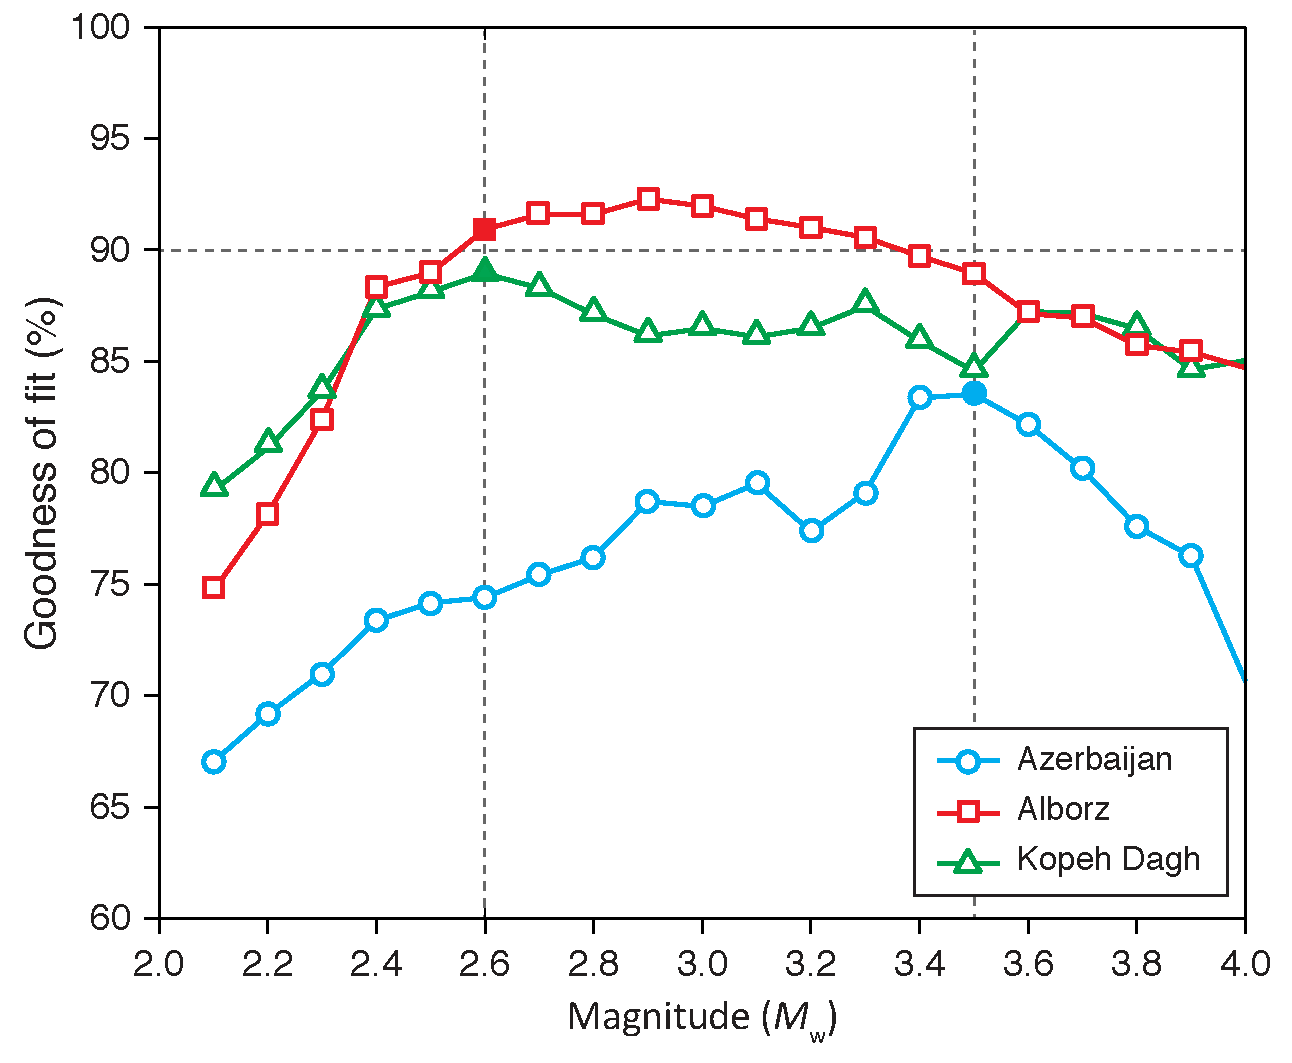
\includegraphics[width=\textwidth]{figures/pdf/figure-04} 
	\caption{\myrevision{Completeness magnitude, $M_c$, as a function of time (in years) for the three seismic zones in the region of interest, corresponding to the time-magnitude sequences of earthquakes during the 2005--2016 period.}}
	\label{fig:completeness}
\end{figure*}

\myrevision{Subsequently, we} obtained the $b$-value in the Gutenberg-Richter law for each region following the maximum likelihood estimation \citep{Aki1965}, in which
% 
\begin{equation}
\myrevision{
	b = \frac
		{ log_{10}(e) }
		{ \overline{M} - \left( M_{\min} - \frac{\Delta M_{\mathrm{bin}}}{2} \right) } \, ,
}
\end{equation}
%
\noindent%
where $e$ is the mathematical constant or Euler's number, $\overline{M}$ is the average magnitude, \myrevision{$M_{\min}$ is the minimum magnitude in the sample, and $\Delta M_{\mathrm{bin}}$ is the bin size used to discretize the magnitude scale}. Here, the value of $M_{\min}$ is taken as the minimum completeness magnitude $M_c$ obtained or selected for each region's sub-catalog. \myrevision{In this study we assumed $\Delta M_{\mathrm{bin}} = 0.1$}. 

In addition to using $M_c$ to determine $b$ for each sub-catalog, we also use it as the threshold for limiting the minimum magnitude to be considered in the construction of the visibility graphs for each region. \myrevision{Table \ref{tab:seismicity} shows the number of events of the whole catalog, along with the number of events for each region's complete and declustered catalogs. It also includes the corresponding values of $M_c$, which happened to be the same for both catalogs, and the separate values of $b$, including the standard deviation, $\sigma_b$, which is calculated as}
% 
\begin{equation}
\myrevision{
	\sigma_b = 2.3 \, b^2 \sqrt{ \frac{ \sum_{i = 1}^{N} \left( M_i - \overline{M} \right)^2 }{ N \left(N - 1 \right) } } \, ,
}
\end{equation}
% 
\noindent
where $N$ is the number of events in each catalog \citep{Shi1982standard}. 

\myrevision{Figure \ref{fig:mag-time} shows the final time-magnitude sequences for the complete catalogs of Azerbaijan, Alborz, and Kopeh Dagh. We omit here the sequences of the declustered catalogs, which are, in general, very similar to those shown in Fig.~\ref{fig:mag-time}. Note from Table \ref{tab:seismicity} that in the case of Azerbaijan and Kopeh Dagh, we consider events in the catalog with $M_w \geq 3.5$, whereas in the case of Alborz all events are $M_w \geq 3.0$.}

\myrevision{
\begin{table*}
	\caption{Total number of earthquakes \myrevision{for the whole, complete, and declustered catalogs}, and seismic parameters $M_c$ and $b$ \myrevision{(including standard deviation) for the complete catalogs} of the three seismic zones of northern Iran.}
	\centering\small
	\myrevision{
	\begin{tabular}{lcccccc}
		\hline
		Region       & \multicolumn{3}{c}{Number of Events in Catalog} & $M_c$ & \multicolumn{2}{c}{$b$-value} \\
		\cline{2-4}\cline{6-7} 
		             & Whole & Complete & Declustered &     & Complete             & Declustered \\
		\hline
		Azerbaijan   & 1047  &  202     &   102       & 3.5 & 0.85491 $\pm$ 0.0506 & 0.88187 $\pm$ 0.07107 \\
		Alborz       & 1898  &  575     &   440       & 3.0 & 0.81578 $\pm$ 0.0279 & 0.78941 $\pm$ 0.030923 \\
		Kopeh Dagh   &  640  &  117     &    96       & 3.5 & 0.78297 $\pm$ 0.0494 & 0.73026 $\pm$ 0.048949 \\
		\hline
	\end{tabular}
	}
	\label{tab:seismicity}
\end{table*}
}

\begin{figure*}%[t]
	\centering
	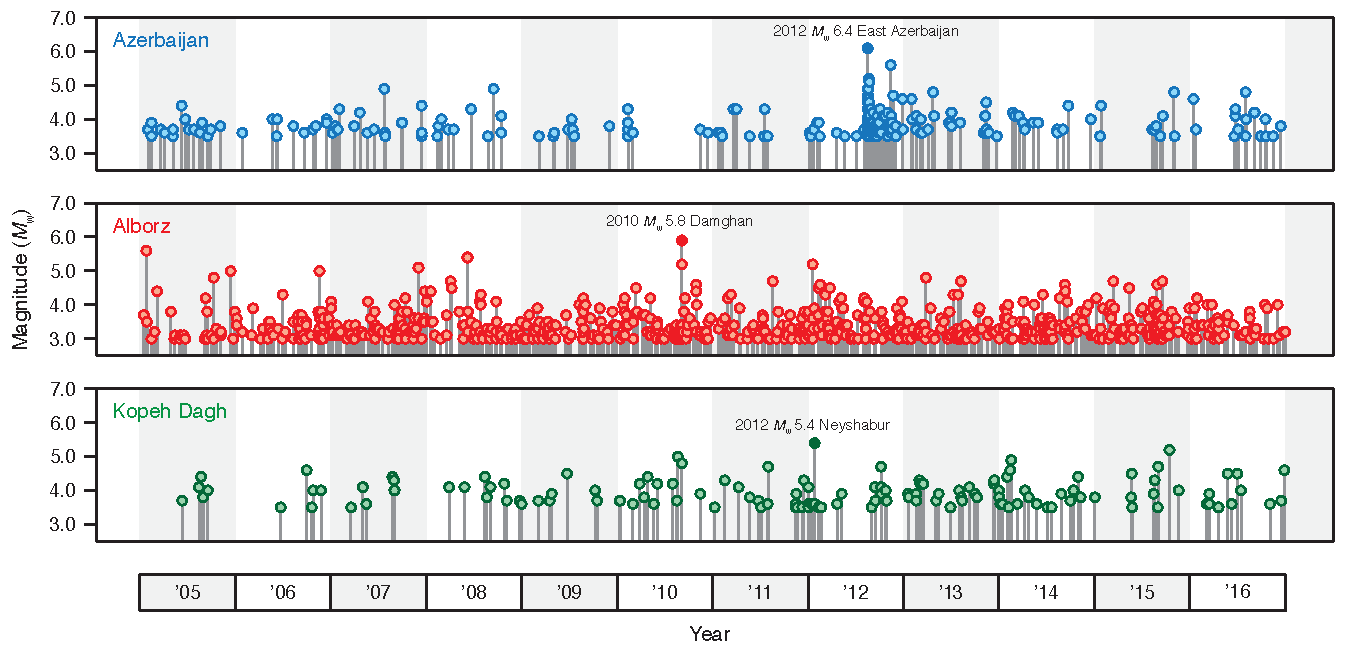
\includegraphics[width=\textwidth]{figures/pdf/figure-05} 
	\caption{Time-magnitude sequences for the northern Iran seismic zones of Azerbaijan, Alborz and Kopeh Dagh, during the period between 1 January 2005 and 31 December \myrevision{2016}. The event occurrences are represented by vertical bars or sticks of length equal to the $M_w$ magnitude of each earthquake. These sequences correspond to the \myrevision{whole} catalog but in each case we consider only events with $M_w \geq M_c$. As shown in Fig.~\ref{fig:vg}, the dots at the top of each stick represent the nodes of the visibility graphs. The edges or links are omitted for visual convenience. Highlighted in the figure are the largest events in each sub-catalog, namely the 2012 $M_w$ 6.4 East Azerbaijan, 2010 $M_w$ 5.8 Damghan, and 2012 $M_w$ 5.4 Neyshabur earthquakes.}
	\label{fig:mag-time}
\end{figure*}

% OLD MATERIAL
% -----------------------------------------------------------------

% \myrevision{After conducting separate studies on the whole and declustered catalog, we found that the whole catalog results are ,although slightly different, comprehensive. On the other hand declustering could add some unwanted uncertainty (in using parameters for time and distance windows) to the resultant catalog and considerably reduce the number of events in each region's catalog}. Fig.~\ref{fig:seismicity} shows the epicenter location of instrumental earthquakes for the three seismic zones of interest.

%Foreshocks and aftershocks were removed from the catalog following a Poissonian occurrence model using the declustering method of \citet{Gardner1974}, in a manner consistent with previous catalog compilations available for the region \citep[e.g.,][]{Zare2014}. Upon declustering, we divide the catalog into three sub-catalogs, each for one of the seismic zones under consideration. 

% We 
% \cmmnt{then proceeded to} 
% determine the minimum magnitude of completeness, $M_c$, for each region's sub-catalog. The value of $M_c$ is often determined using simple numerical analyses in combination with data inspection. Two common approaches are the maximum curvature (MAXC) and the goodness-of-fit test (GFT) methods \citep{Wiemer2001}. \myrevision{We compute the $M_c$ versus time using the \myrevision{MAXC} 
% \cmmnt{GFT} 
% method coded in ZMAP software} as introduced by \citet{Wiemer2000}. 

% \cmmnt{In this method, the completeness magnitude is obtained such that the catalog satisfies---at a certain acceptance threshold---the Gutenberg-Richter power low, given an extended dataset of events. This extended dataset is composed of predicted and observed events, where the predicted events are generated based on a trial minimum magnitude. The process is repeated for increasing values of the reference minimum magnitude until finding a desirable fit with the power law. \citet{Wiemer2000} suggests a goodness of fit of 90\% as an acceptable threshold to select $M_c$. However, not all frequency-magnitude distributions reach the 90\% mark, in which case $M_c$ can be selected by inspection.} 

% Figure \ref{fig:completeness} shows the 
% % \cmmnt{goodness-of-fit} 
% \myrevision{$M_c$ vs time} values for the three seismic zones. We indicate the selected value of $M_c$ for each region in the figure. 

% \cmmnt{
% \begin{figure}%[t]
% 	\centering
% 	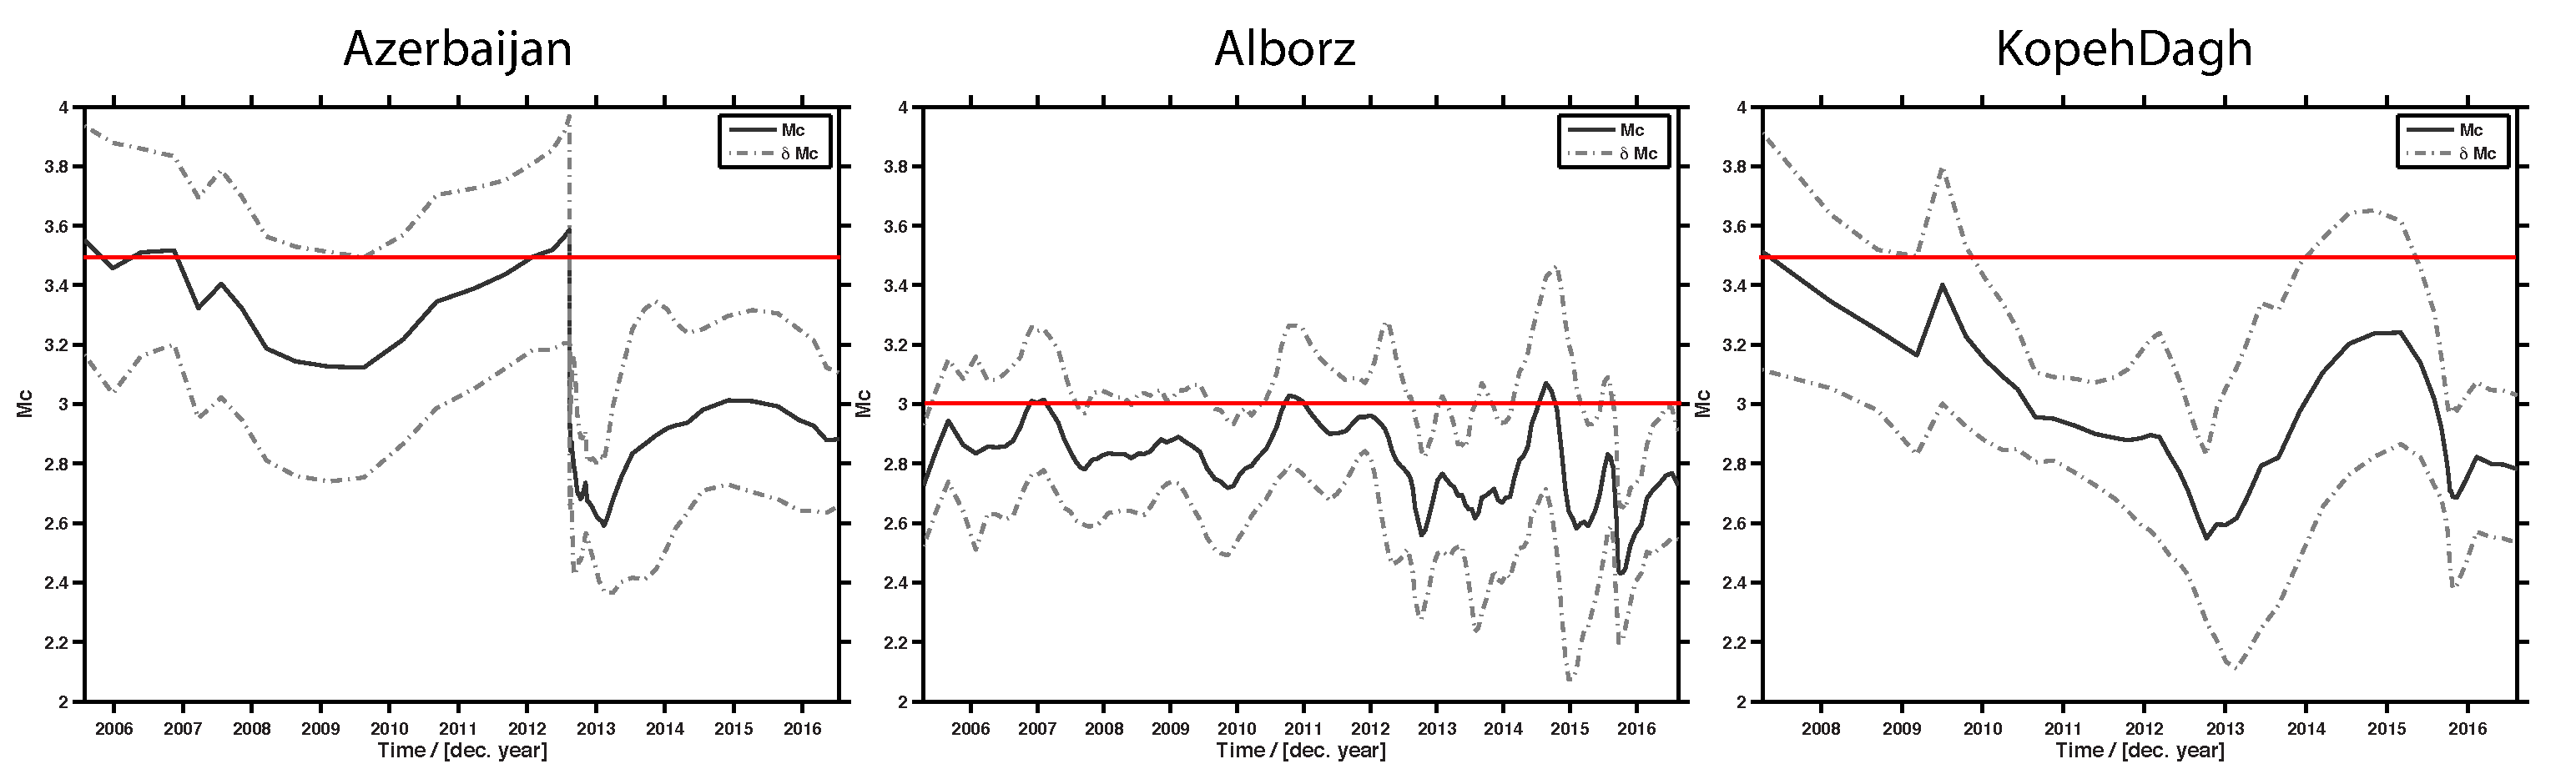
\includegraphics[width=0.45\textwidth]{figures/pdf/figure-04-rev} 
% 	\caption{Completeness magnitude goodness-of-fit test (GFT) results and selected $M_c$ values for the three tectonic seismic regions in northern Iran as evaluated from the time-magnitude sequence of earthquakes during the 2005--2015 period. The symbols indicate the computed GFT values as function of the earthquake magnitude. The horizontal dashed line indicates the desired threshold for the GFT value at 90 percent. The vertical dashed lines and solid symbols indicate the selected completeness magnitude for each region. The color version of this figure is available only in the electronic edition.}
% 	\label{fig:completeness}
% \end{figure} 
% }


